\documentclass{article}

% Symbols
\usepackage{amsfonts, amsthm}
\usepackage{upgreek}
\usepackage{physics}
\usepackage{cancel}
\usepackage{amssymb, latexsym, amsmath}

%Algorithms
\usepackage[ruled,lined,linesnumbered,commentsnumbered]{algorithm2e}

%% Identación
\setlength{\parindent}{0cm}

% Código
\newcommand{\code}[1]{\textcolor{white!25!black}{\texttt{#1}}}
\usepackage{listings}

%AMS
\usepackage{amsthm}
\newtheorem{algo-thm}{Algoritmo}

% Proof
\renewcommand*{\proofname}{\textbf{Demostraci\'on:}}
% Theorem
\newtheorem*{theorem}{Teorema}

% Graphics
\usepackage{graphicx}
\usepackage{pgf}

% Color a letras.
%\usepackage[usenames,dvipsnames,svgnames,table]{xcolor}

% Tikz
\usepackage{tkz-graph}
\usepackage{tikz}
\usetikzlibrary{arrows,automata}
\usepackage{tikz}
\usetikzlibrary{arrows,automata}
%\usetikzlibrary[topaths]

% Margins
\addtolength{\voffset}{-1.5cm}
\addtolength{\hoffset}{-1.5cm}
\addtolength{\textwidth}{3cm}
\addtolength{\textheight}{3cm}

%Header-Footer
\usepackage{fancyhdr}
\renewcommand{\headrulewidth}{1pt}

\newcommand{\set}[1]{
  \left\{ #1 \right\}
}

%\pagenumbering{gobble} -- Este comando
%                       -- quita el número de página.
\footskip = 50pt
\renewcommand{\headrulewidth}{1pt}

\pagestyle{fancyplain}

\begin{document}
\title{UNIVERSIDAD AUT\'ONOMA DE M\'EXICO\\ Facultad de Ciencias}
\author{Autor: Adri\'an Aguilera Moreno}
\date{}
\maketitle
\begin{center}
  
\includegraphics[scale=0.20]{../Imagen/Portada.jpg}\\[0.4cm]
  \Large
  \bf{Aut\'omatas y Lenguajes Formales}
  \normalsize
\end{center}
\newpage
\fancyhead[r]{ Aut\'omatas y Lenguajes Formales 2022-2}
%%%%%%%%%%%%%%%%%%%%%%%%%%%%%%%%%%%%%%%%%%%%%%%%%%%%%
\section*{\LARGE{Tarea 1}}
\begin{enumerate}
  %%%%%%%%%%%%%%%%%%%%%%%%%%%%%%%%%%% Ejercicio 01. %%%%%%%%%%%%%%%%%%%%%%%%%%%%%%%%%%%
\item Dados $0 \leq m < k$ y $2 \leq p$, sea
  \[
  A_{k, m, p} = \{a \in \{0, 1, \dotsm, p-1\}^{*} | a
  \text{ es una representación $p$-aria de $x$ y $x\; \mathbf{mod}\; k = m$}\}.
  \]
  Da un método general para construir un autómata que acepte $A_{k, m, p}$.
  
  $\triangledown$ \textbf{Solución:}
  Sea $\alpha$ una cadena $p$-aria, entonces $\#\alpha$ es el
  número que representa a esta cadena en notación decimal. De
  lo anterior se propone la función de transición de cadenas
  \[
  \delta^{*}(0, \alpha) = \#\alpha\; \mathbf{mod}\; k
  \]
  Así, cuando se quiera construir un aut\'omata se debe considerar
  como estado final a los residuos indicados\footnote{En caso de
  pedir que un valor sea m\'ultiplo, el estado terminal debe ser $0$.}
  de manera explícita.
  
  Definimos
  \begin{eqnarray*}
    \#(\alpha d) &=& p \cdot (\#\alpha) + d\\
    \delta(q, d) &=& (pq + d)\; \mathbf{mod}\; k
  \end{eqnarray*}
  donde $d\in{0,1, \dotsm, p - 1}$ es alguna transición y $q$ un estado
  en el autómata.

  Ahora mostremos lo anterior por inducción en $\alpha$ [en la cadena $p$-aria],
  esto es
  \begin{eqnarray*}
    \delta^{*}(0, \lambda) &=& 0
    \hspace*{3.3cm} \text{Por definición de } \delta.\\
    &=& \#\lambda
    \hspace*{3.4cm} \text{Pues } \#\lambda = 0.\\
    &=& \#\lambda\; \mathbf{mod}\; k
    \hspace*{1.3cm} \text{Sabemos que } 0\; mod\; k = 0.
  \end{eqnarray*}
  y como se puede ver, la cadena vacia cumple con nuestra definición.
  Ahora, supongamos sin pérdida de generalidad que nuestra condición
  se cumple para alguna cadena $p$-aria $\mu$, \textit{i.e.}
  \[
  \delta^{*}(0, \mu) = \#\mu\; \mathbf{mod}\; k
  \hspace*{1cm} \text{H.I.}
  \]
  veamos que pasa con la cadena $\mu d$, donde $d \in \{0, 1, \dotsm, p - 1\}$, así
  \begin{eqnarray*}
    \delta^{*}(0, \mu) &=& \delta(\delta^{*}(0, \mu), d)
    \hspace*{2.5cm} \text{Definición alternativa de }\delta^{*}.\\
    &=& \delta(\# \mu\; \mathbf{mod}\; k, d)
    \hspace*{2.3cm} \text{Hipótesis de inducción.}\\
    &=& (p \cdot (\#\mu\; \mathbf{mod}\; k) + d)\; \mathbf{mod}\; k
    \hspace*{1cm} \text{Definición de }\delta.\\
    &=& (p \cdot \#\mu + d)\; \mathbf{mod}\; k
    \hspace*{2cm} \text{Teoría de Números.}\\
    &=& \# \mu d\; \mathbf{mod}\; k
    \hspace*{2.4cm} \text{Definición dada previamente.}
  \end{eqnarray*}
  Ahora, veamos un ejemplo de esta construcción:
  
  \hspace*{0.4cm} ``Diseña un autómata que acepte números en
  notación ternaria que al ser divididos entre $3$ dejen residuo
  de $2$''. Resolviendo tenemos que: Sea $A_{3, 2, 3}$ un autómata
  tal que resuelve el problema anteriormente planteado, así el
  estado terminal (en este caso, el único estado terminal) es $2$.
  
  Observemos los primeros $15$ valores en notación terciaria
  \begin{eqnarray*}
    &0 - 0 \hspace*{2cm} 11 - 4 \hspace*{2cm} 22 - 8 \hspace*{2cm} 110 - 12&\\
    &1 - 1 \hspace*{2cm} 12 - 5 \hspace*{2cm} 100 - 9 \hspace*{2cm} 111 - 13&\\
    &2 - 2 \hspace*{2cm} 20 - 6 \hspace*{2cm} 101 - 10 \hspace*{1.8cm} 112 - 14&\\
    &10 - 3 \hspace*{1.9cm} 21 - 7 \hspace*{2cm} 102 - 11 \hspace*{1.9cm} 120 - 15&
  \end{eqnarray*}
  esto nos ayudará a encontrar las transiciones (al usar $\delta$ con
  algunas de estas cadenas terciarias).

  Veamos en la siguiente tabla la relación de módulos con $k = 3$:
  \begin{center}
    \begin{tabular}{| c | c |}
      \hline
      Expresión & Residuo \\ \hline
      $0\; \mathbf{mod}\; 3$ & 0 \\
      $1\; \mathbf{mod}\; 3$ & 1 \\
      $2\; \mathbf{mod}\; 3$ & 2\\
      $3\; \mathbf{mod}\; 3$ & 0\\\hline
    \end{tabular} 
  \end{center}
  Nótese que
  \[
  0\; \mathbf{mod}\; 3 \equiv 3\; \mathbf{mod}\; 3
  \]
  por tanto consideraremos solo los tres primeros casos,
  también es claro que la columna de Residuos son los estados
  en $A_{3, 2, 3}$. A continuación se muestra la tabla de
  transición de $A_{3, 2, 3}$:
  \begin{center}
    \begin{tabular}{| c | c | c | c |}
      \hline
      $\mathbf{Q}$ & $\mathbf{0}$ & $\mathbf{1}$ & $\textcircled{2}$\\ \hline
      $\rightarrow \mathbf{0}$ & 0 & 1 & 2 \\
      $\mathbf{1}$ & 0 & 1 & 2 \\
      $\mathbf{2}$ & 0 & 1 & 2 \\\hline
    \end{tabular} 
  \end{center}
  \textbf{Obs.} En este caso ``$\rightarrow \mathbf{0}$'' indica el estado inicial
  en el autómata, mientras que $\textcircled{2}$ indica el estado terminal.

  Así, podemos comprobar la información en la tabla de transición por medio de la
  función $\delta^{*}$, esto es
  \begin{eqnarray*}
    &\;\;\delta(0) = 0 \hspace*{2cm} \;\delta^{*}(11) = 1
    \hspace*{2cm} \delta^{*}(22) = 2 \hspace*{2cm} \;\;\delta^{*}(110) = 0&\\
    &\;\;\delta(1) = 1 \hspace*{2cm} \;\delta^{*}(12) = 2
    \hspace*{2cm} \delta^{*}(100) = 0 \hspace*{2cm} \delta^{*}(111) = 1&\\
    &\;\;\delta(2) = 2 \hspace*{2cm} \delta^{*}(20) = 0
    \hspace*{2cm} \delta^{*}(101) = 1 \hspace*{1.8cm} \;\;\delta^{*}(112) = 2&\\
    &\delta^{*}(10) = 0 \hspace*{1.9cm} \delta^{*}(21) = 1
    \hspace*{1.8cm} \delta^{*}(102) = 2 \hspace*{1.9cm} \;\;\delta^{*}(120) = 0&
  \end{eqnarray*}
  Por último, veamos la representación de $A_{3,2,3}$ como una gráfica de estados
  \begin{center}
    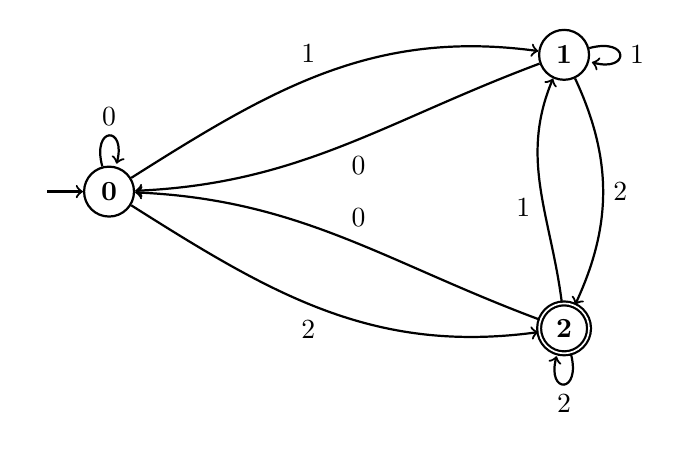
\begin{tikzpicture}[estado/.style={circle,draw=black},auto,/tikz/initial text={},
        final/.style={circle,draw=black,double},thick]
      \node [estado,initial] (0) [right=0pt, left = 45]   {$\mathbf{0}$};
      \node [estado]         (1) [right=110pt,above=40pt] {$\mathbf{1}$};
      \node [estado,final]   (2) [right=110pt,below=40pt] {$\mathbf{2}$};
      \path[->]
      (0) edge [curve to, out=15,in=155,relative] node {1} (1)
          edge [loop above] node {0} (0)
      (1) edge [curve to, out=3,in=165,relative] node {0} (0)
      (0) edge [curve to, out=-15,in=-155,relative] node [swap] {2} (2)
      (2) edge [curve to, out=-3,in=-165,relative] node [swap] {0} (0)
      (1) edge [curve to, out=25,in=155,relative] node {2} (2)
          edge [loop right] node {1} (1)
      (2) edge [curve to, out=5,in=155,relative] node {1} (1)
          edge [loop below] node {2} (2);
    \end{tikzpicture}
  \end{center}
  \hfill $\lhd$
  \newpage
  %%%%%%%%%%%%%%%%%%%%%%%%%%%%%%%%%%% Ejercicio 02. %%%%%%%%%%%%%%%%%%%%%%%%%%%%%%%%%%%  
\item Transforma el siguiente autómata no determinista con transiciones-$\varepsilon$
  en uno determinista usando los métodos vistos en clase.
  \begin{center}
    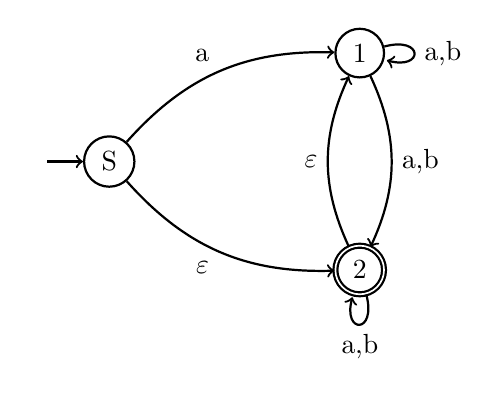
\begin{tikzpicture}[estado/.style={circle,draw=black},auto,/tikz/initial text={},
        final/.style={circle,draw=black,double},thick]
      \node [estado,initial] (S) [right=0pt] {S};
      \node [estado]         (1) [right=100pt,above=30pt] {1};
      \node [estado,final]   (2) [right=100pt,below=30pt] {2};
      \path[->]
      (S) edge [curve to, out=25,in=155,relative] node {a} (1)
      (S) edge [curve to, out=-25,in=-155,relative] node [swap] {$\varepsilon$} (2)
      (1) edge [curve to, out=25,in=155,relative] node {a,b} (2)
      edge [loop right] node {a,b} (1)
      (2) edge [curve to, out=25,in=155,relative] node {$\varepsilon$} (1)
      edge [loop below] node {a,b} (2);
    \end{tikzpicture}
  \end{center}
  $\triangledown$ \textbf{Solución:} Sea $A_{\varepsilon} = \langle Q, \Sigma, \Delta, S, F\rangle$
  el autómata representado por la gráfica de estados anterior, y sea $Q = \{S,1,2\}$
  el conjunto de estados, entonces
  \[
  \mathcal{P}(Q) = \{\phi, \{S\}, \{1\}, \{2\}, \{S,1\}, \{S,2\}, \{1,2\}, \{S,1,2\}\}
  \]
  Definamos $A = \langle Q_{D}, \Sigma, \delta_{D}, s_D, F_D\rangle$ cuya gráfica de
  estados se presenta a continuación
  \begin{center}
    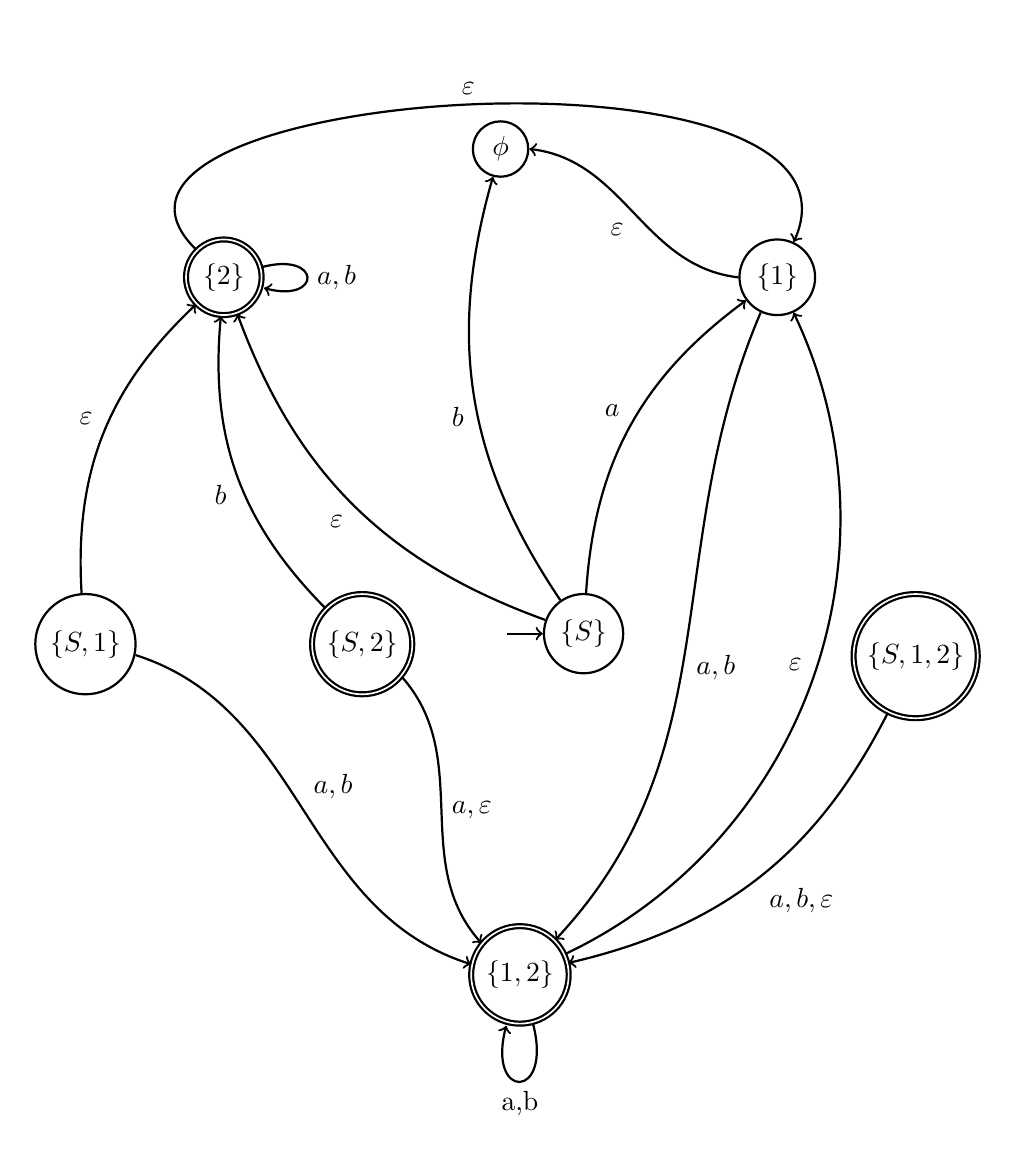
\begin{tikzpicture}[estado/.style={circle,draw=black},auto,/tikz/initial text={},
        final/.style={circle,draw=black,double},thick]
      \node [estado,initial] (S) [right=30pt,  below=0pt]    {$\{S\}$};
      \node [estado]         (0) [right=0pt,   above=150pt]  {$\phi$};
      \node [estado]         (1) [right=100pt, above=100pt]  {$\{1\}$};
      \node [estado]        (s1) [left=150pt,  below=0pt]    {$\{S,1\}$};
      \node [estado,final]   (2) [left=100pt,  above=100pt]  {$\{2\}$};
      \node [estado,final]  (s2) [left=50pt,   below=0pt]    {$\{S,2\}$};
      \node [estado,final]  (12) [right=7pt,   below=120pt]  {$\{1,2\}$};
      \node [estado,final] (s12) [right=150pt, below=0pt]    {$\{S,1,2\}$};
      \path[->]
      (S) edge [curve to, out=25,in=155,relative] node {$b$} (0)
      (S) edge [curve to, out=25,in=155,relative] node {$a$} (1)
      (s2) edge [curve to, out=25,in=155,relative] node {$b$} (2)
      (1) edge [curve to, out=-5,in=155,relative] node {$a, b$} (12)
      (s1) edge [curve to, out=25,in=-155,relative] node {$a, b$} (12)
      (S) edge [curve to, out=25,in=155,relative] node {$\varepsilon$} (2)
      (s1) edge [curve to, out=25,in=155,relative] node {$\varepsilon$} (2)
      (1) edge [curve to, out=25,in=-155,relative] node {$\varepsilon$} (0)
      (2) edge [curve to, out=135,in=-295,relative] node {$\varepsilon$} (1)
      edge [loop right] node {$a,b$} (2)
      (12) edge [curve to, out=-45,in=-135,relative] node {$\varepsilon$} (1)
      edge [loop below] node {a,b} (12)
      (s2) edge [curve to, out=25,in=-155,relative] node {$a, \varepsilon$} (12)
      (s12) edge [curve to, out=25,in=155,relative] node {$a, b, \varepsilon$} (12);
    \end{tikzpicture}
  \end{center}
  Ahora, veamos las transiciones a través de la función $\delta_{D}$ [que como sabemos,
    existe una equivalencia $\delta_{D} = \Delta^{*} = \Delta^{*}_{\varepsilon}$], así
  \begin{center}
    \begin{tabular}{ c  c  c }
      $\Delta^{*}_{\varepsilon}\left(\{S\}, \varepsilon\right) = \{2\}$ & $\Delta^{*}_{\varepsilon}\left(\{S\}, a\right) = \{1\}$
      & $\Delta^{*}_{\varepsilon}\left(\{S\}, b\right) = \phi$\\
      $\Delta^{*}_{\varepsilon}\left(\{1\}, \varepsilon\right) = \phi$  & $\Delta^{*}_{\varepsilon}\left(\{1\}, a\right) = \{1,2\}$
      & $\Delta^{*}_{\varepsilon}\left(\{1\}, b\right) = \{1,2\}$ \\
      $\Delta^{*}_{\varepsilon}\left(\{2\}, \varepsilon\right) = \{1\}$ & $\Delta^{*}_{\varepsilon}\left(\{2\}, a\right) = \{2\}$
      & $\Delta^{*}_{\varepsilon}\left(\{2\}, b\right) = \{2\}$\\
      $\Delta^{*}_{\varepsilon}\left(\{1,2\}, \varepsilon\right) = \{1\}$ & $\Delta^{*}_{\varepsilon}\left(\{1,2\}, a\right) = \{1,2\}$
      & $\Delta^{*}_{\varepsilon}\left(\{1,2\}, b\right) = \{1,2\}$ \\
      $\Delta^{*}_{\varepsilon}\left(\{S,1\}, \varepsilon\right) = \{2\}$ & $\Delta^{*}_{\varepsilon}\left(\{S,1\}, a\right) = \{1,2\}$
      & $\Delta^{*}_{\varepsilon}\left(\{S,1\}, b\right) = \{1,2\}$ \\
      $\Delta^{*}_{\varepsilon}\left(\{S,2\}, \varepsilon\right) = \{1,2\}$ & $\Delta^{*}_{\varepsilon}\left(\{S,2\}, a\right) = \{1,2\}$
      & $\Delta^{*}_{\varepsilon}\left(\{S,2\}, \varepsilon\right) = \{2\}$ \\
      $\Delta^{*}_{\varepsilon}\left(\{S,1,2\}, \varepsilon\right) = \{1,2\}$ & $\Delta^{*}_{\varepsilon}\left(\{S,1,2\}, a\right) = \{1,2\}$
      & $\Delta^{*}_{\varepsilon}\left(\{S,1,2\}, \varepsilon\right) = \{1,2\}$\\
    \end{tabular} 
  \end{center}
  Por último se presenta la tabla de transiciones del autómata $A$:
  \begin{center}
    \begin{tabular}{| c | c | c | c | c | c | c | c | c |}
      \hline
      $\mathbf{Q}$ & $\mathbf{\{S\}}$ & $\phi$ & $\mathbf{\{1\}}$ & final: $\mathbf{\{2\}}$ & final: $\mathbf{\{1,2\}}$ & $\mathbf{\{S,1\}}$ & final: $\mathbf{\{S,2\}}$ & final: $\mathbf{\{S, 1, 2\}}$\\ \hline
      $\rightarrow \mathbf{\{S\}}$ & -- & b & a & $\varepsilon$ & -- & -- & -- & -- \\ \hline
      $\phi$  & -- & -- & -- & -- & -- & --  & -- & -- \\ \hline
      $\mathbf{\{1\}}$  & -- & $\varepsilon$ & -- & -- & $a, b$ & --  & -- & -- \\\hline
      $\mathbf{\{2\}}$  & -- & -- & $\varepsilon$ & $a,b$ & -- & --  & -- & -- \\\hline
      $\mathbf{\{1,2\}}$  & -- & -- & $\varepsilon$ & -- & $a,b$ & -- & -- & -- \\\hline
      $\mathbf{\{S,1\}}$  & -- & -- & -- & $\varepsilon$ & $a,b$ & -- & -- & -- \\\hline
      $\mathbf{\{S,2\}}$  & -- & -- & -- & $b$ & $a, \varepsilon$ & -- & -- & --  \\\hline
      $\mathbf{\{S,1,2\}}$  & -- & -- & -- & -- & $a,b,\varepsilon$ & --  & -- & -- \\\hline
    \end{tabular} 
  \end{center}
  \hfill $\lhd$
  %%%%%%%%%%%%%%%%%%%%%%%%%%%%%%%%%%% Ejercicio 03. %%%%%%%%%%%%%%%%%%%%%%%%%%%%%%%%%%%  
\item Construye un autómata que acepte el lenguaje generado por la expresión regular siguiente
  \[
  (1 + 1(0^{*}1)^{*}1)^{*} + (0^{*}1^{*} + (10)^{*})
  \]
  $\triangledown$ \textbf{Solución:}
  
  \hfill $\lhd$
\end{enumerate}
\end{document}
